This section presents the proposed business model for introducing \textit{HydroTracker} to the market as a product for the service industry. It includes a Business Canvas that outlines the value proposition, key cost and revenue activities, as well as a demonstration video showing the functionality of the \textit{HydroTracker}, and a promotional video.

\subsection{Business Canvas}
The \textit{HydroTracker} is an innovative water level monitoring system designed to improve customer experience and support staff efficiency in the service industry. It enables quick and efficient refills of water, helping staff respond quickly to customer needs and avoid missed requests during peak hours. This not only improves the overall customer experience, but also supports better task coordination among staff, resulting in a less stressful work environment.

What makes \textit{HydroTracker} stand out is its ability to integrate smoothly into existing service processes. Its compatibility with PDA order management systems enhances operational efficiency while reinforcing the business’s professional image. 

The primary costs in this business model include the sourcing of sensors and micro-controllers, prototype production, software development, and promotional activities.

The target market consists of approximately 110,000 service industry businesses in Greece, with early adopters being futuristic and luxury venues aiming for premium service. In the future, cost reductions will allow expansion to small and medium-sized business owners, as well as exports. Additionally, thanks to its modular and scalable architecture, \textit{HydroTracker} can be extended beyond cafés—such as into office spaces, hospitals, or co-working environments—offering smart hydration 

\begin{figure}[H]
    \centering
    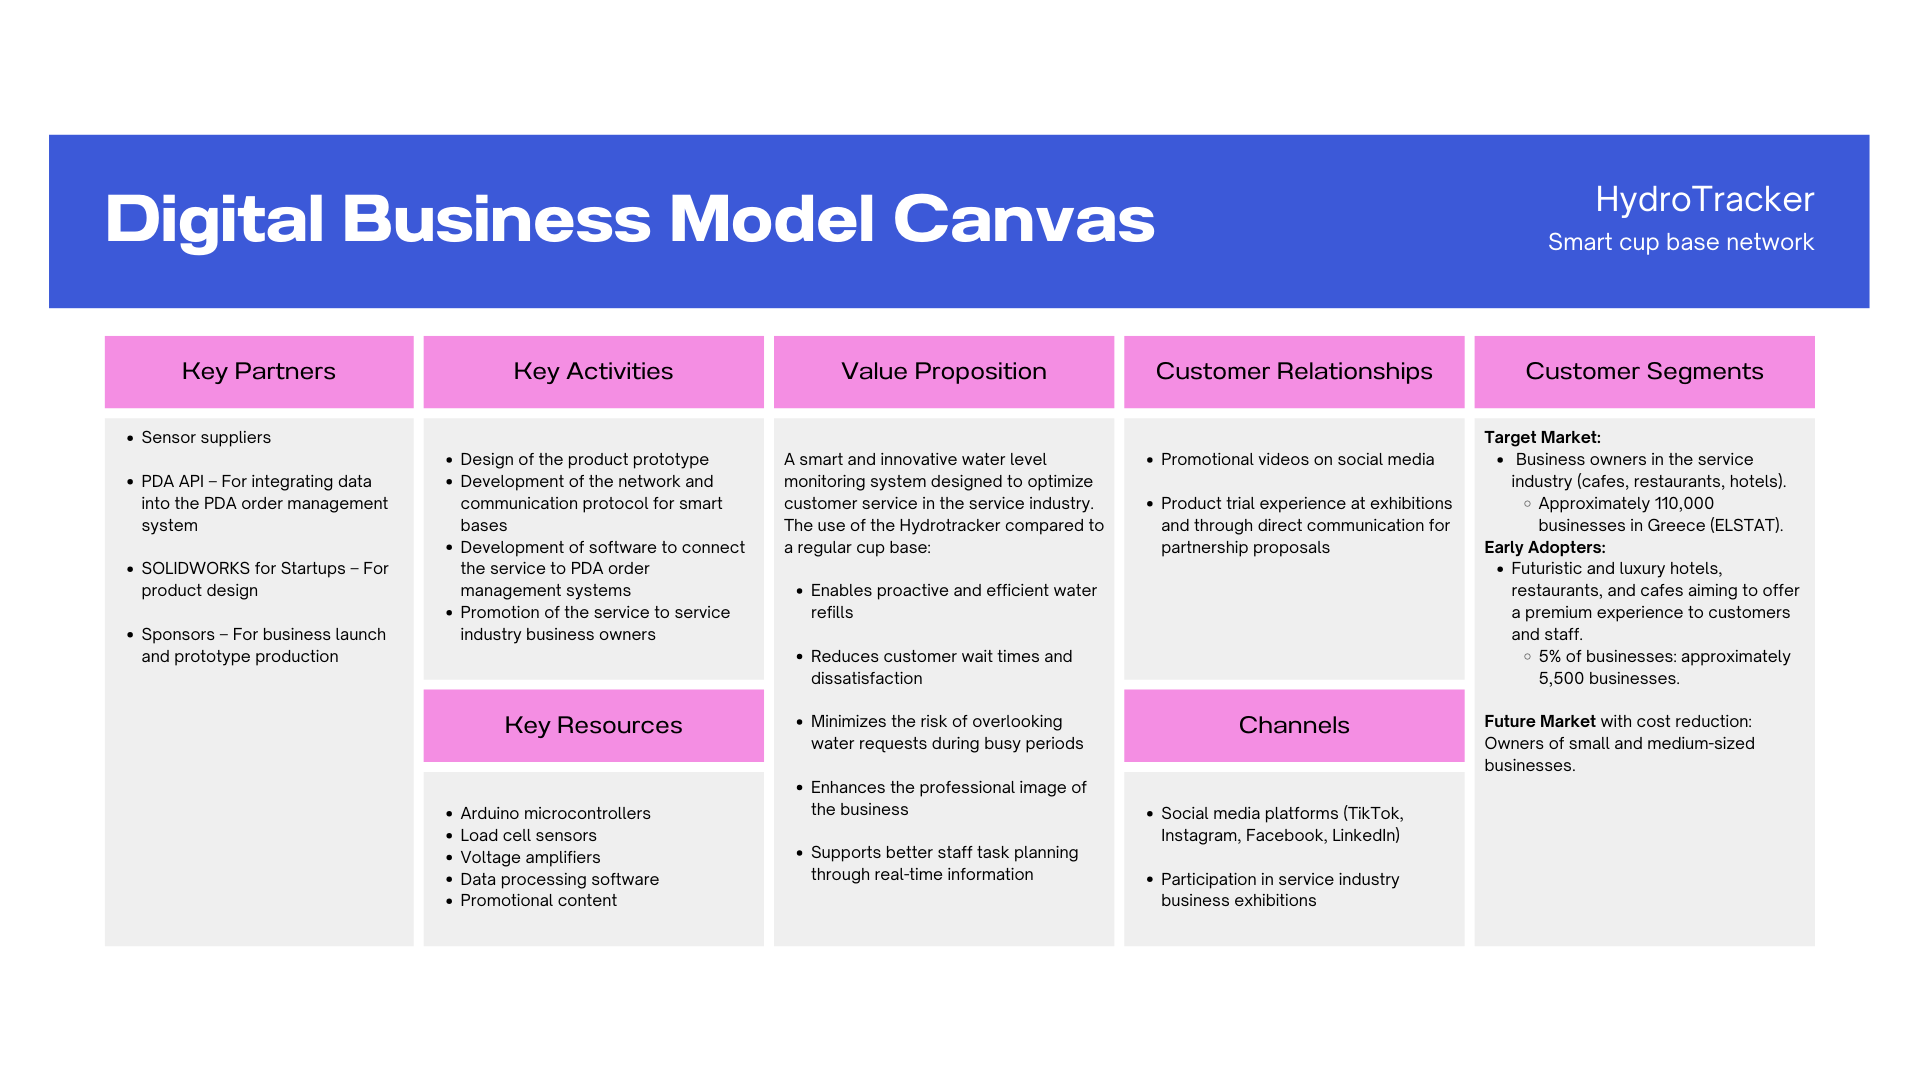
\includegraphics[width=\linewidth]{assets\business_images\HydroTracker - Business Canvas.png}
    \caption{\textit{HydtroTracker} Business Canvas}
    \label{fig:enter-label}
\end{figure}

\subsection{Demonstration Video}
A demonstration video showcasing the functionality of the \textit{HydroTracker} is available \href{https://youtu.be/DthdfglUvXY?si=8oIWrk7Wovcrerfg}{here}. The video presents how the system operates in a real-world setting, highlighting its key features.

\subsection{Promotional Video}
A promotional video has been created to highlight the key benefits of the HydroTracker for potential customers and investors. The video is available \href{https://www.youtube.com/watch?v=uHeOhnM9qX0}{here}.